\documentclass[a4paper]{article}
\usepackage{amsmath}
\usepackage{amssymb}
\usepackage{graphicx}
\usepackage{a4wide}
\usepackage{url}
\usepackage{pdfpages}

\usepackage{natbib} 
\citestyle{aa}
\bibpunct{(}{)}{;}{a}{}{,}

\newcommand{\mytilde}{\raise.17ex\hbox{$\scriptstyle\mathtt{\sim}$}}
\setlength{\parindent}{0pt}

% Listings to import code into LaTeX
\usepackage{listings}
\usepackage{color}
\usepackage{textcomp}
\definecolor{listinggray}{gray}{0.9}
\definecolor{lbcolor}{rgb}{0.9,0.9,0.9}
\lstset{
	backgroundcolor=\color{lbcolor},
	tabsize=4,
	rulecolor=,
	language=bash,
        basicstyle=\scriptsize,
        upquote=true,
        aboveskip={1.5\baselineskip},
        columns=fixed,
        showstringspaces=false,
        extendedchars=true,
        breaklines=true,
        prebreak = \raisebox{0ex}[0ex][0ex]{\ensuremath{\hookleftarrow}},
        frame=single,
        showtabs=false,
        showspaces=false,
        showstringspaces=false,
        identifierstyle=\ttfamily,
        keywordstyle=\color[rgb]{0,0,1},
        commentstyle=\color[rgb]{0.133,0.545,0.133},
        stringstyle=\color[rgb]{0.627,0.126,0.941},
}
% End of Listings

\begin{document}
\begin{figure}[h!] 
\begin{center} 

\includegraphics{UvA_Logo_Image_EN.jpg} \\

\includegraphics{UvA_Logo_Text_EN.jpg} \\

\includegraphics{API_Logo_Text.pdf} 
\end{center} 
\end{figure} 

\begin{center}
\line(1,0){420} \\
\huge \textbf{Basic Linux and Coding for AA (BLAC) \\ Exercise 3 (week 2)} \\
\line(1,0){420}
\end{center}

\vfill

%\begin{figure}[h!] 
%\begin{center} 
%\includegraphics[width=12cm]{graphgraphMyGraph} 
%\end{center} 
%\end{figure} 
%\addtocounter{figure}{-1} % start counting at figure 1 again


\begin{table}[h]
\begin{center}
\begin{tabular}{lp{5cm}l}
\textit{Author:} & & \emph{Supervisor:} \\
Timo Halbesma, 6126561 & & Dr. T. Coenen\\
\end{tabular}
\end{center}
\end{table}

% End of titlepage

\newpage

\lstinputlisting[caption={TLRH's solution for the BLAC homework 3 (week 2) \label{list:hw1}}]{../Week2/knmi-1-6126561.py}


%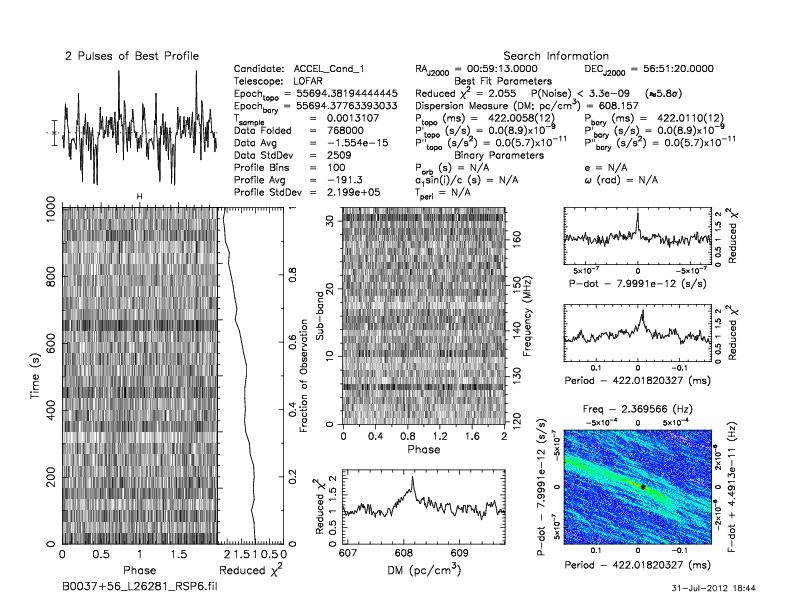
\includepdf[pages=-]{Brightest.png}
% ../Exercise1/L26281_RSP6/B0037+56_L26281_RSP6_DM608.36_Z0_ACCEL_Cand_1.png


\end{document}